\section{Comparison of my TDL convergence to the references}
\begin{frame}
    \frametitle{Complete comparison}
    \begin{figure}
        \centering
        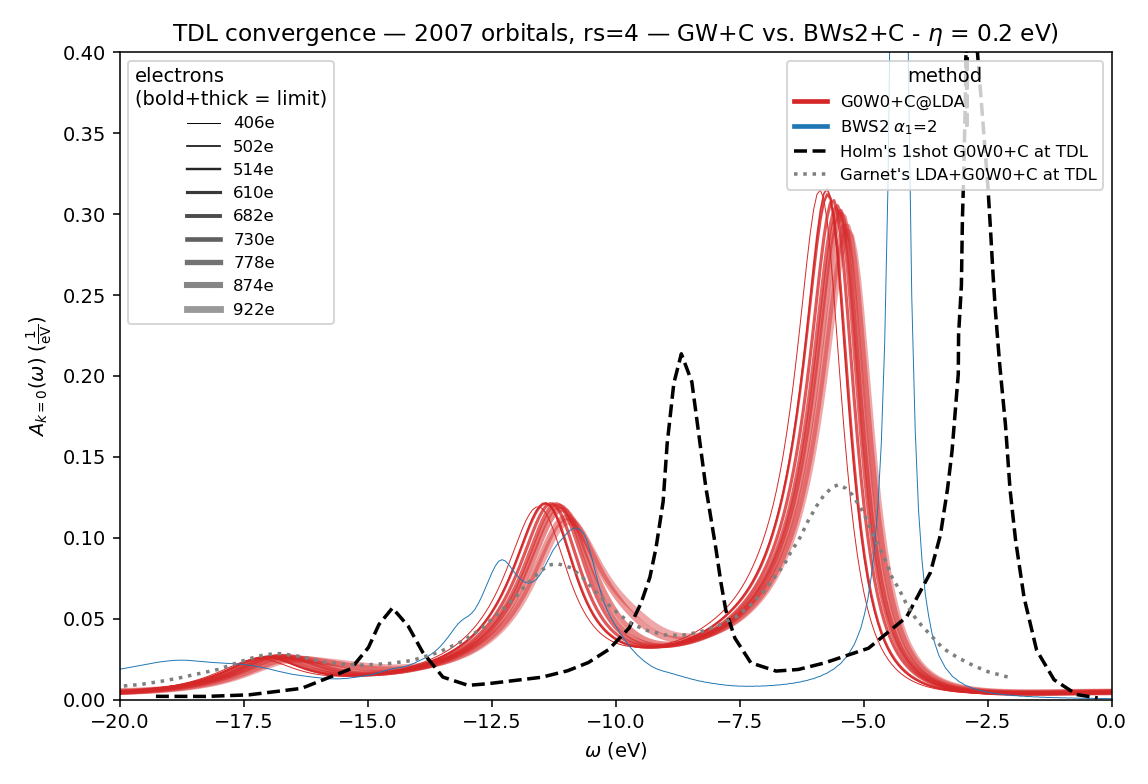
\includegraphics[width=\textwidth]{26/7/7-23/tdl_2007o_joint.png}
        % \caption{LDA+GW}
    \end{figure}
\end{frame}
\begin{frame}
    \frametitle{PPMs}
    \begin{figure}
        \centering
        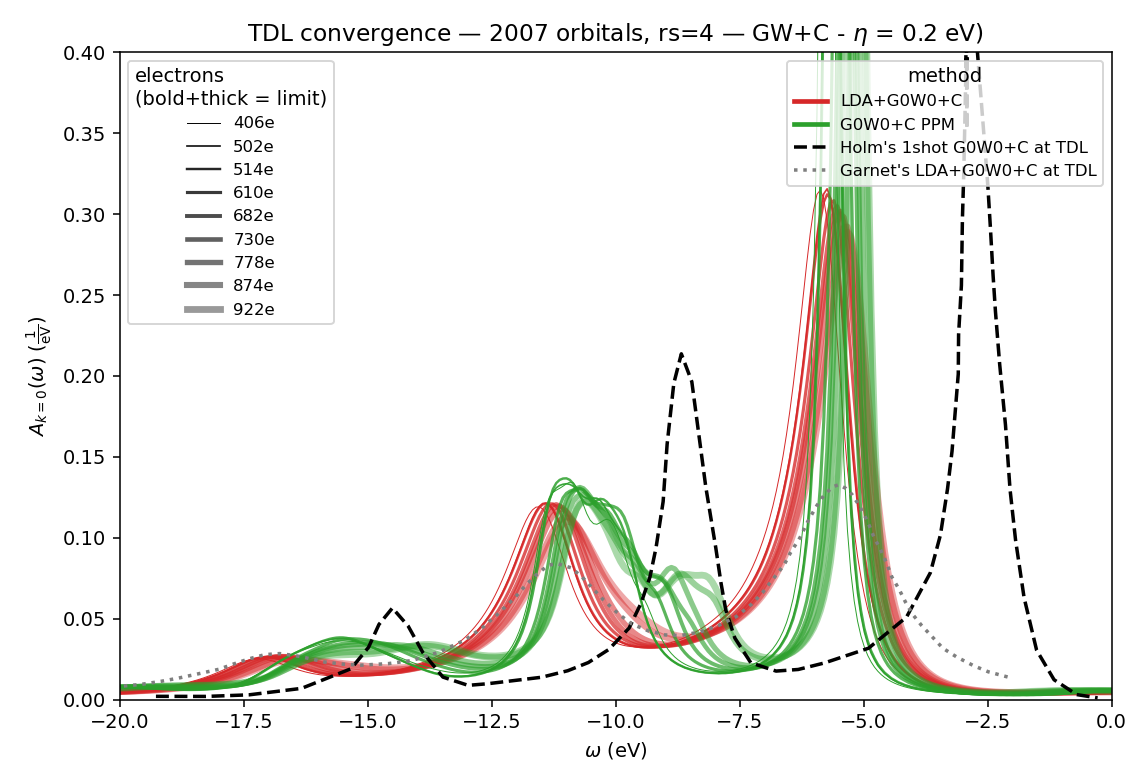
\includegraphics[width=\textwidth]{26/7/7-23/tdl_2007o_gw.png}
        % \caption{LDA+GW}
    \end{figure}
\end{frame}
\section{Assessing TDL convergence through the dielectric function}
\begin{frame}
    \frametitle{406e2007o}
    \begin{figure}
        \centering
        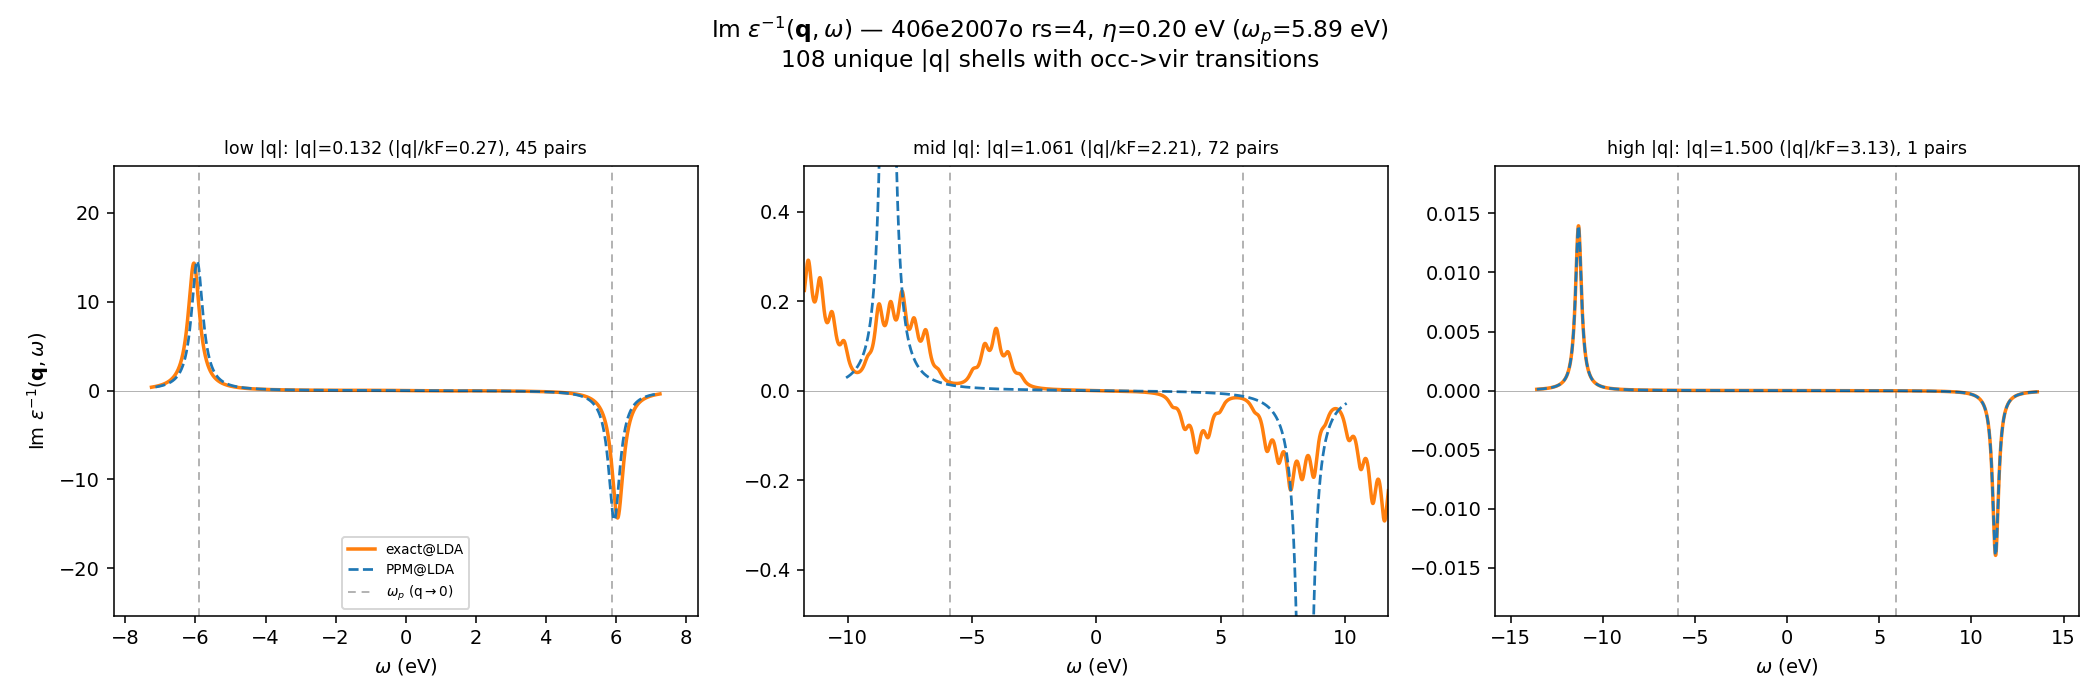
\includegraphics[width=\textwidth]{26/7/7-23/dielectric_406e2007o_im.png}
        % \caption{LDA+GW}
    \end{figure}
\end{frame}
\begin{frame}
    \frametitle{502e2007o}
    \begin{figure}
        \centering
        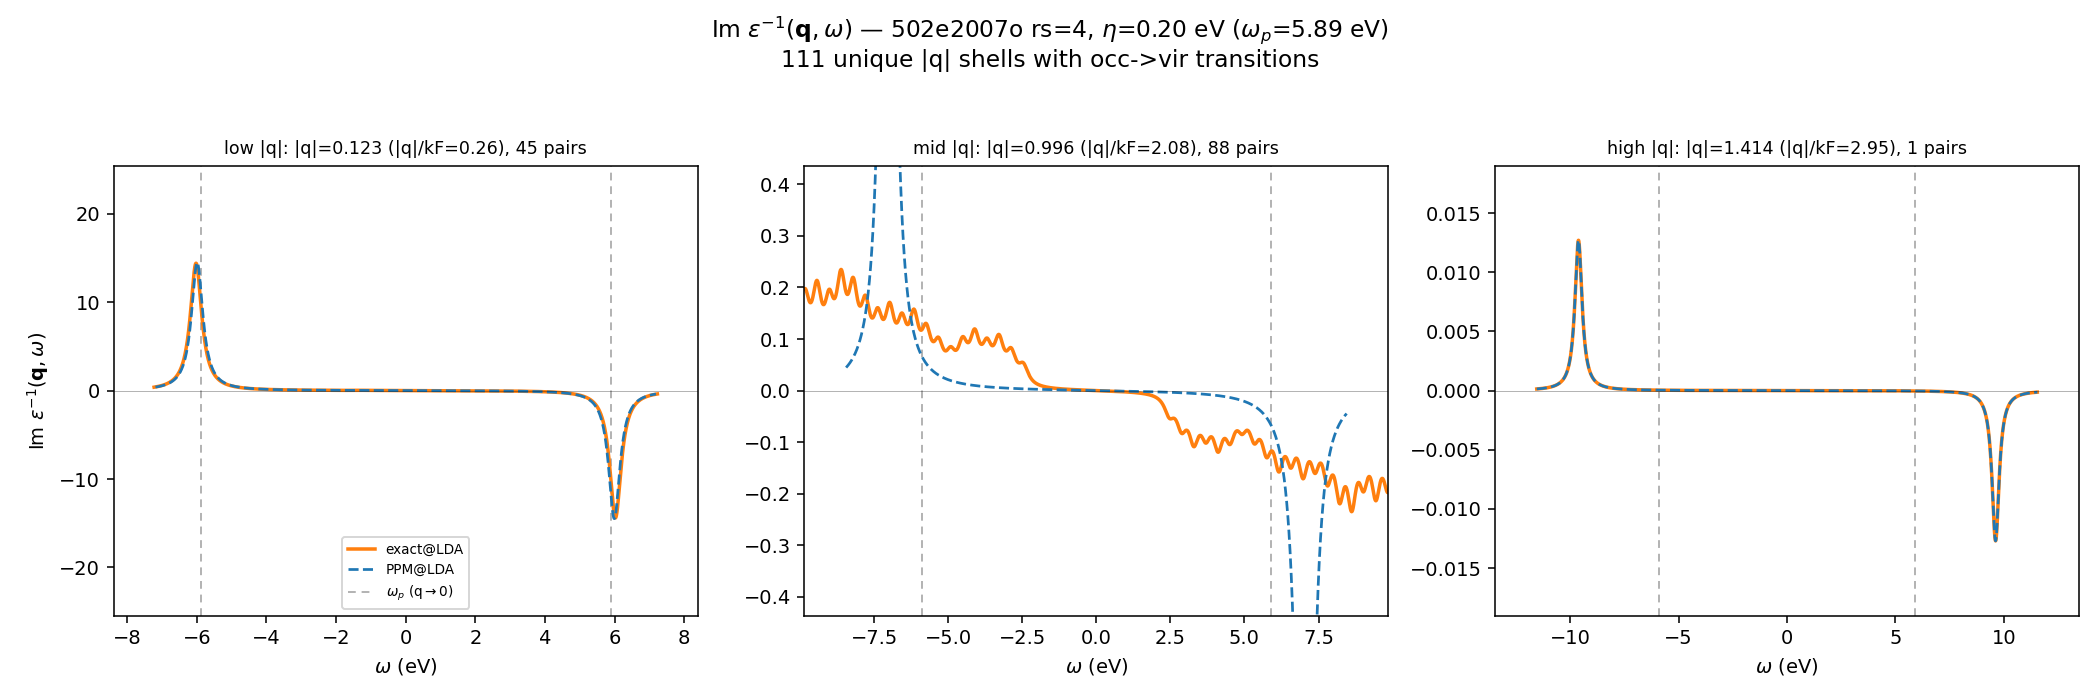
\includegraphics[width=\textwidth]{26/7/7-23/dielectric_502e2007o_im.png}
        % \caption{LDA+GW}
    \end{figure}
\end{frame}
\begin{frame}
    \frametitle{514e2007o}
    \begin{figure}
        \centering
        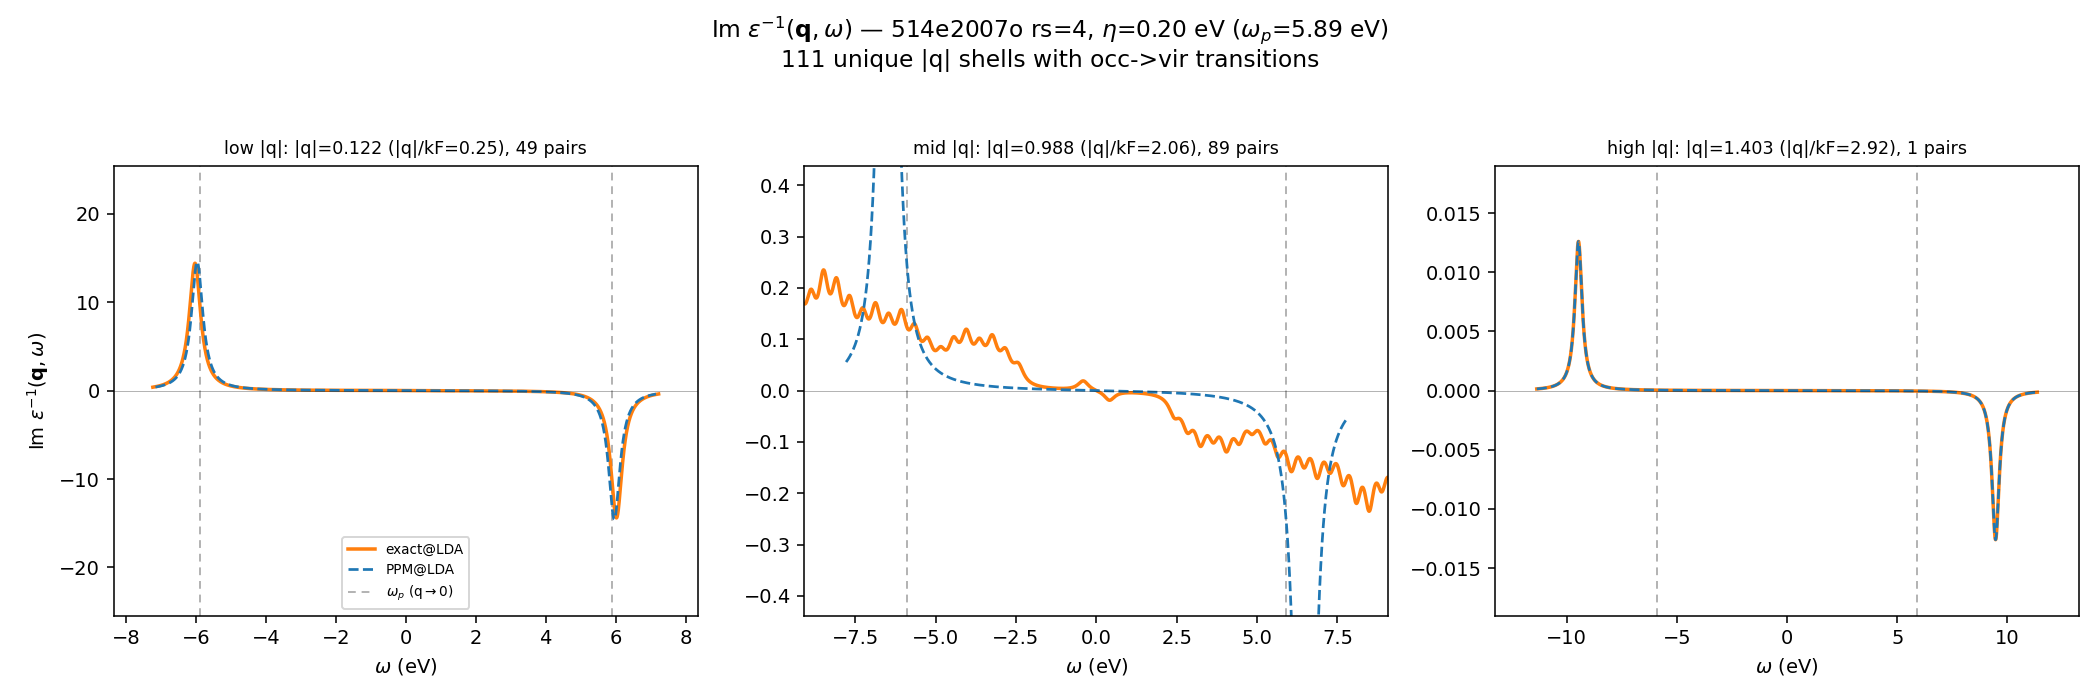
\includegraphics[width=\textwidth]{26/7/7-23/dielectric_514e2007o_im.png}
        % \caption{LDA+GW}
    \end{figure}
\end{frame}
% We have 406, 502, 514, 610, 682, 730, 778, 874, and 922. 
\begin{frame}
    \frametitle{610e2007o}
    \begin{figure}
        \centering
        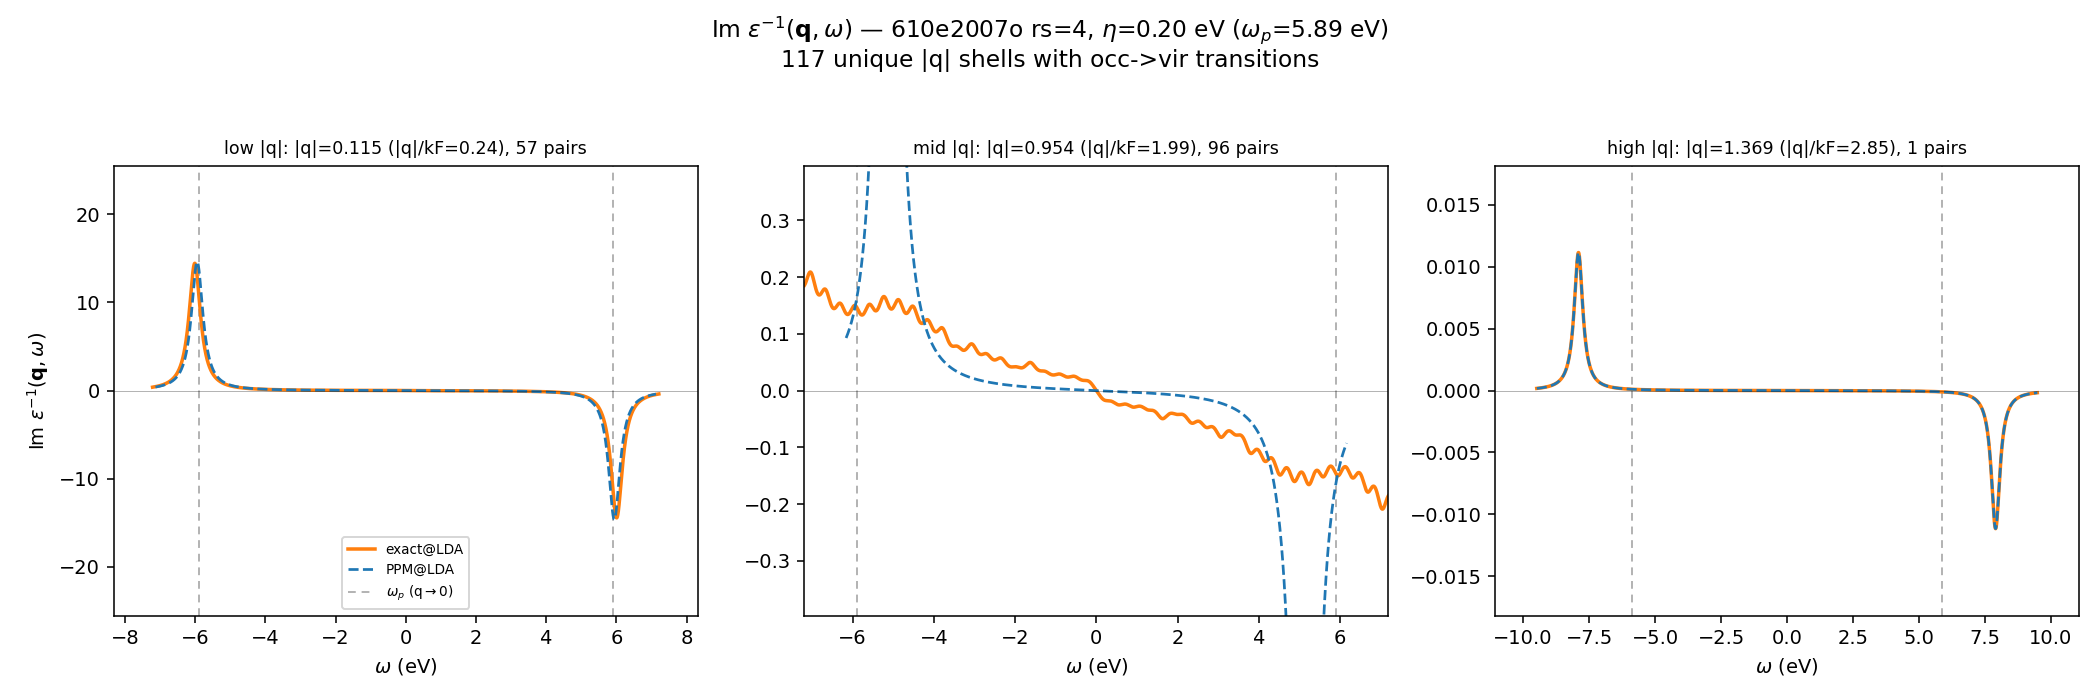
\includegraphics[width=\textwidth]{26/7/7-23/dielectric_610e2007o_im.png}
        % \caption{LDA+GW}
    \end{figure}
\end{frame}
\begin{frame}
    \frametitle{682e2007o}
    \begin{figure}
        \centering
        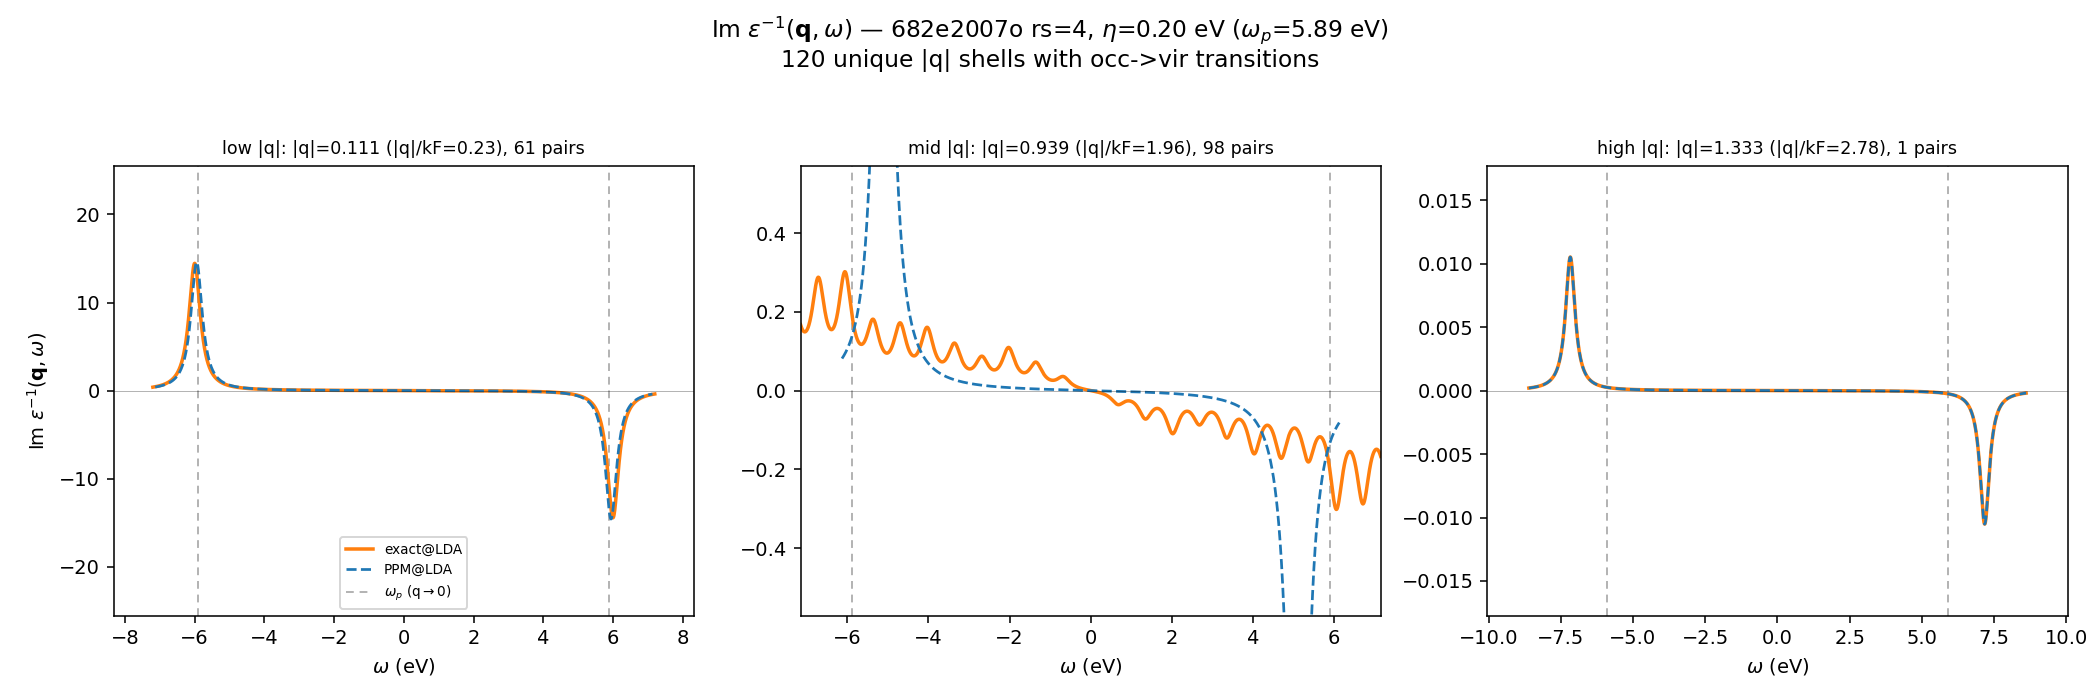
\includegraphics[width=\textwidth]{26/7/7-23/dielectric_682e2007o_im.png}
        % \caption{LDA+GW}
    \end{figure}
\end{frame}
\begin{frame}
    \frametitle{730e2007o}
    \begin{figure}
        \centering
        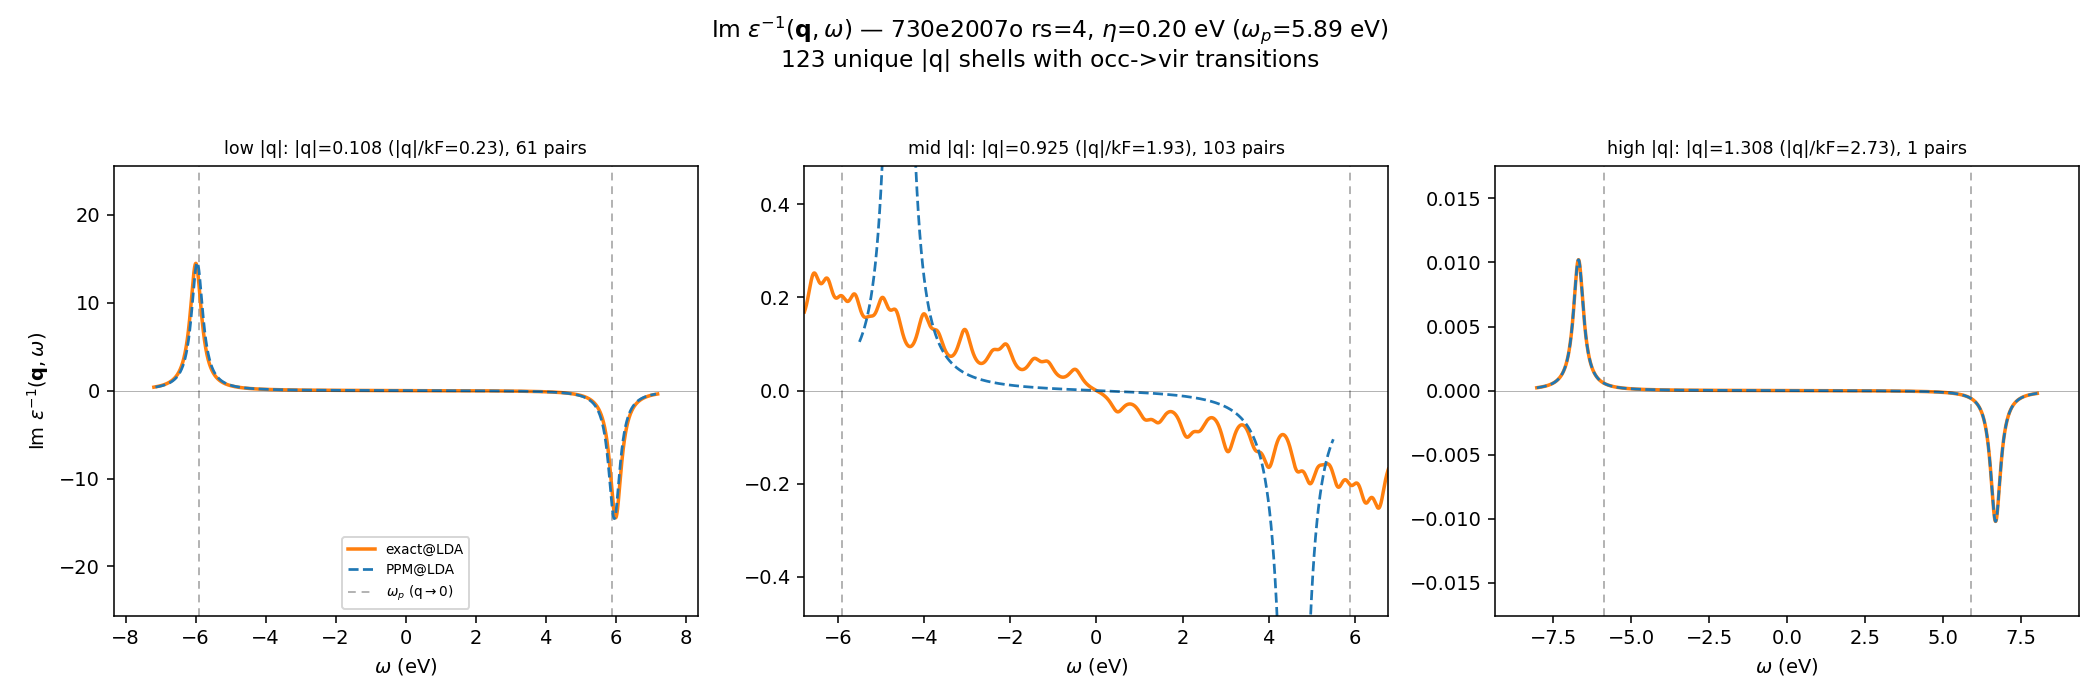
\includegraphics[width=\textwidth]{26/7/7-23/dielectric_730e2007o_im.png}
        % \caption{LDA+GW}
    \end{figure}
\end{frame}
\begin{frame}
    \frametitle{778e2007o}
    \begin{figure}
        \centering
        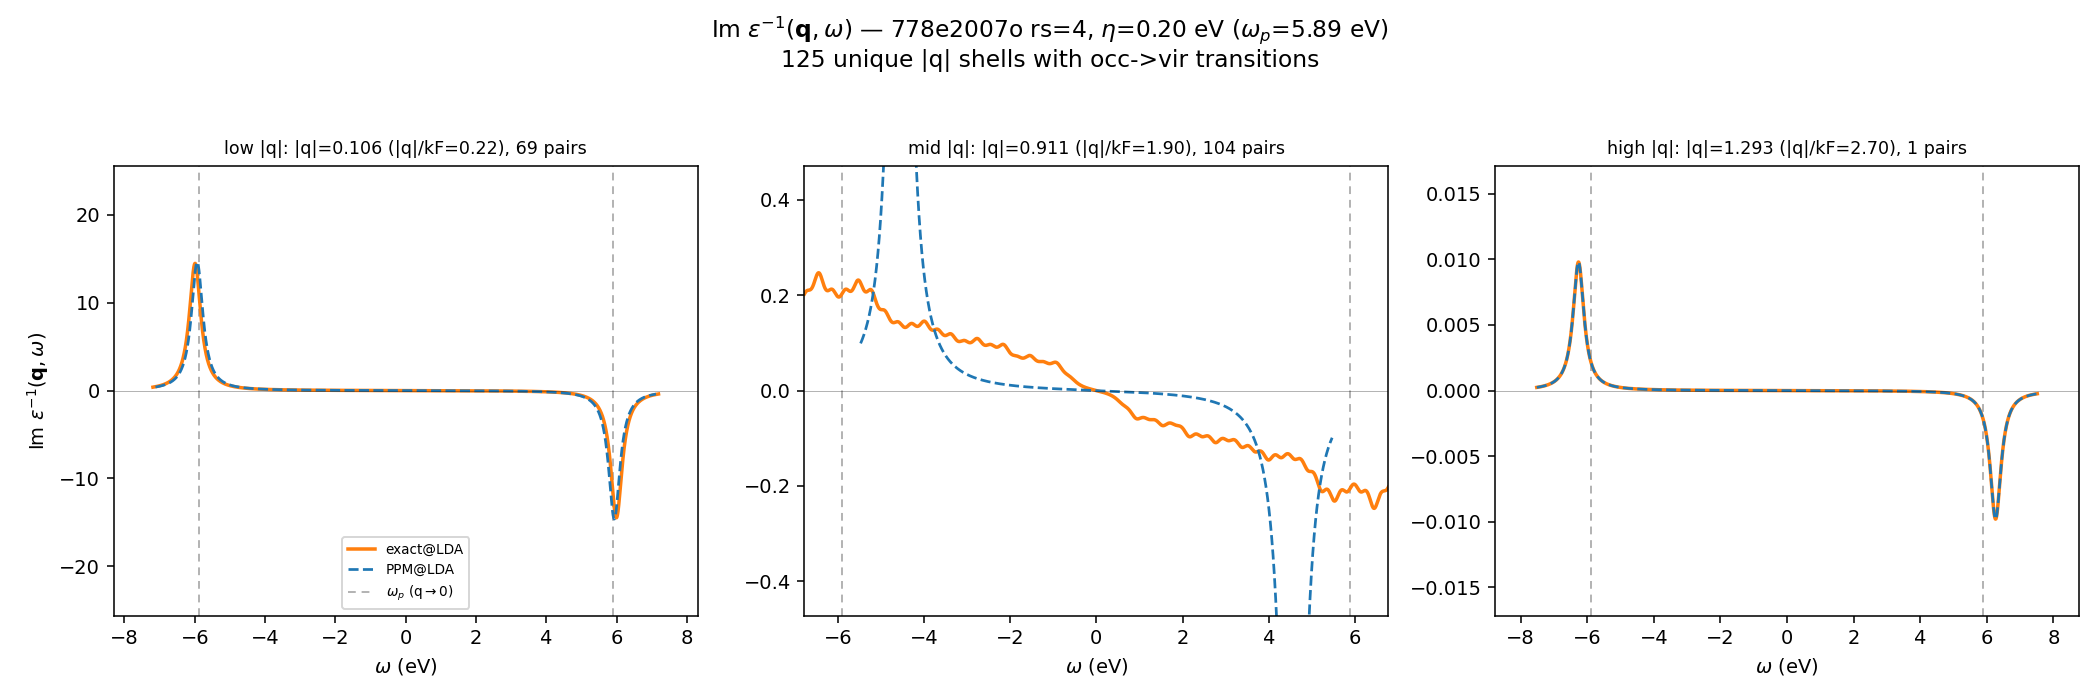
\includegraphics[width=\textwidth]{26/7/7-23/dielectric_778e2007o_im.png}
        % \caption{LDA+GW}
    \end{figure}
\end{frame}
\begin{frame}
    \frametitle{874e2007o}
    \begin{figure}
        \centering
        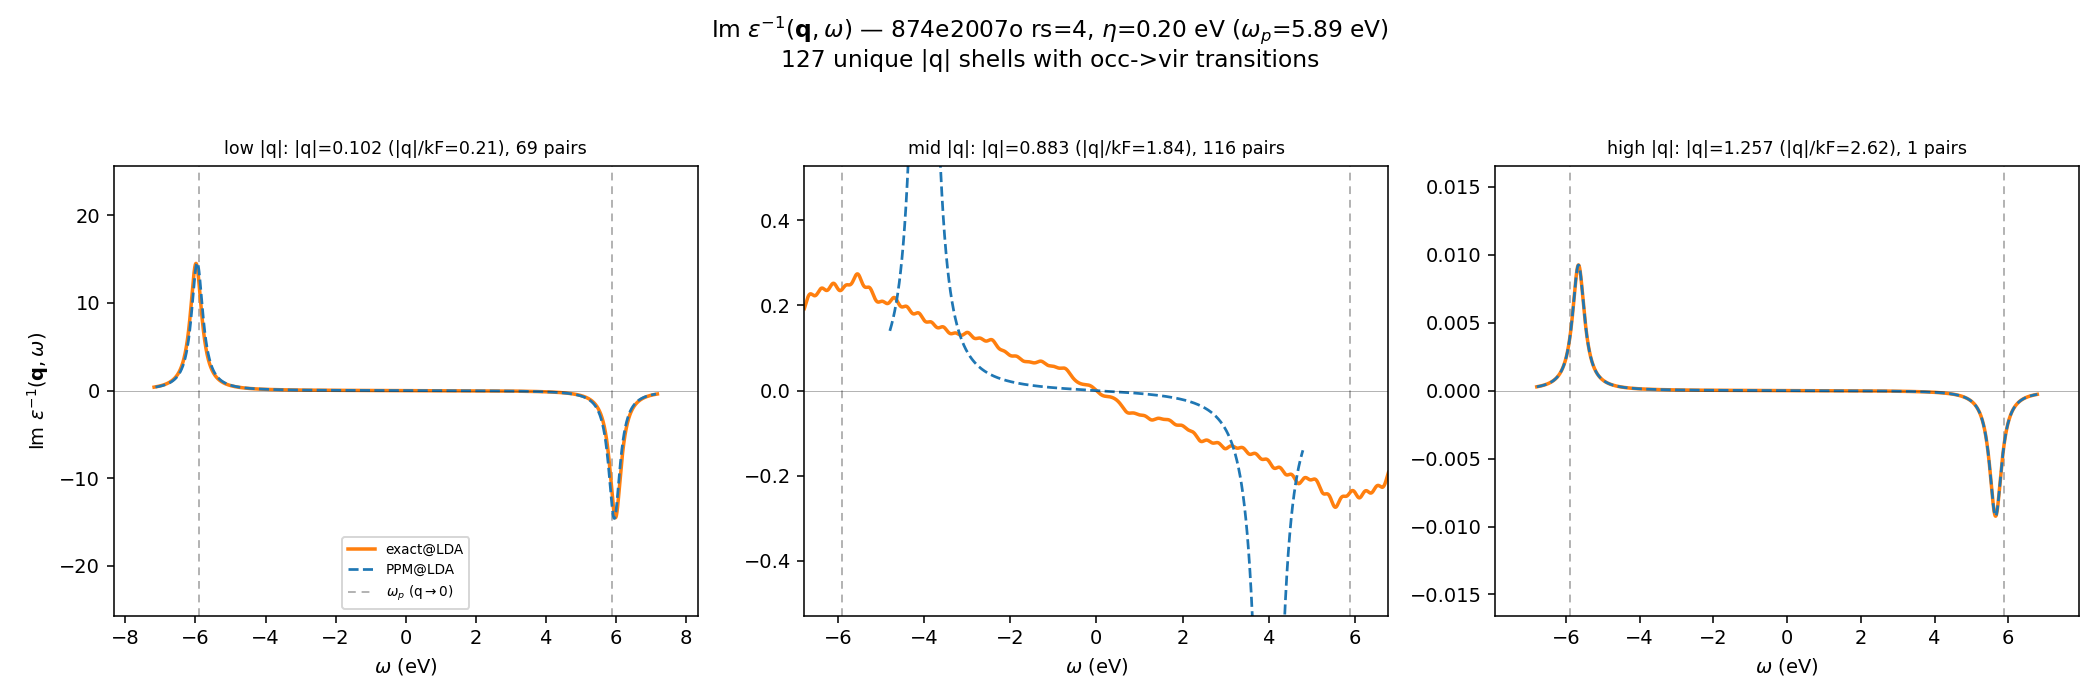
\includegraphics[width=\textwidth]{26/7/7-23/dielectric_874e2007o_im.png}
        % \caption{LDA+GW}
    \end{figure}
\end{frame}
\begin{frame}
    \frametitle{922e2007o}
    \begin{figure}
        \centering
        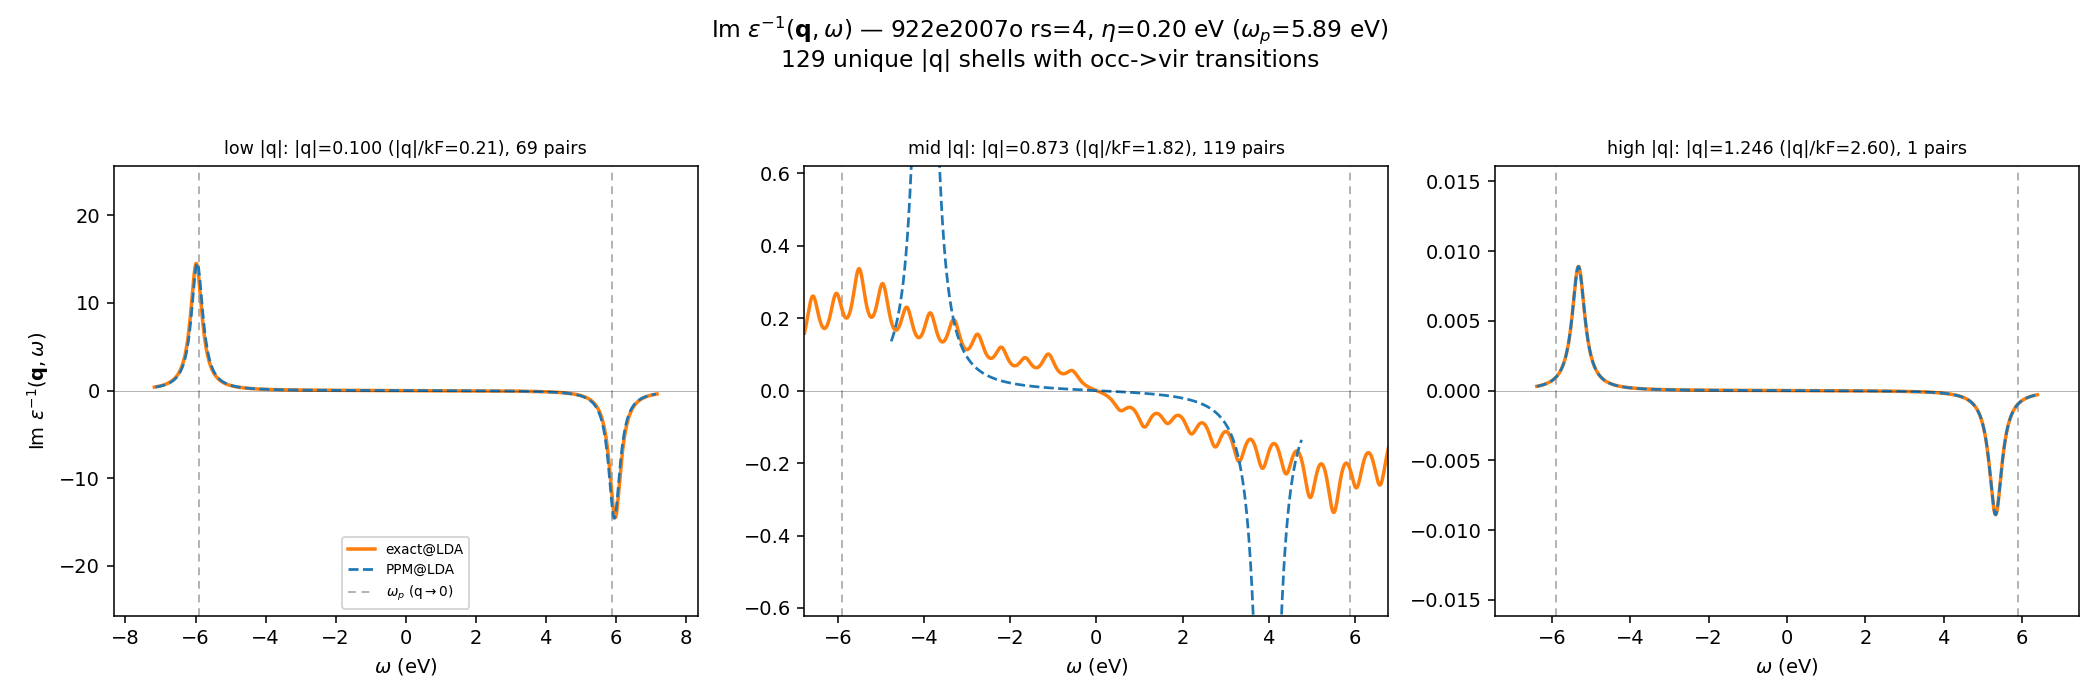
\includegraphics[width=\textwidth]{26/7/7-23/dielectric_922e2007o_im.png}
        % \caption{LDA+GW}
    \end{figure}
\end{frame}
\section{Revisiting things I have done before}
\begin{frame}
    \frametitle{My previous plots overbroadened BWs2+C}
    \begin{figure}
        \centering
        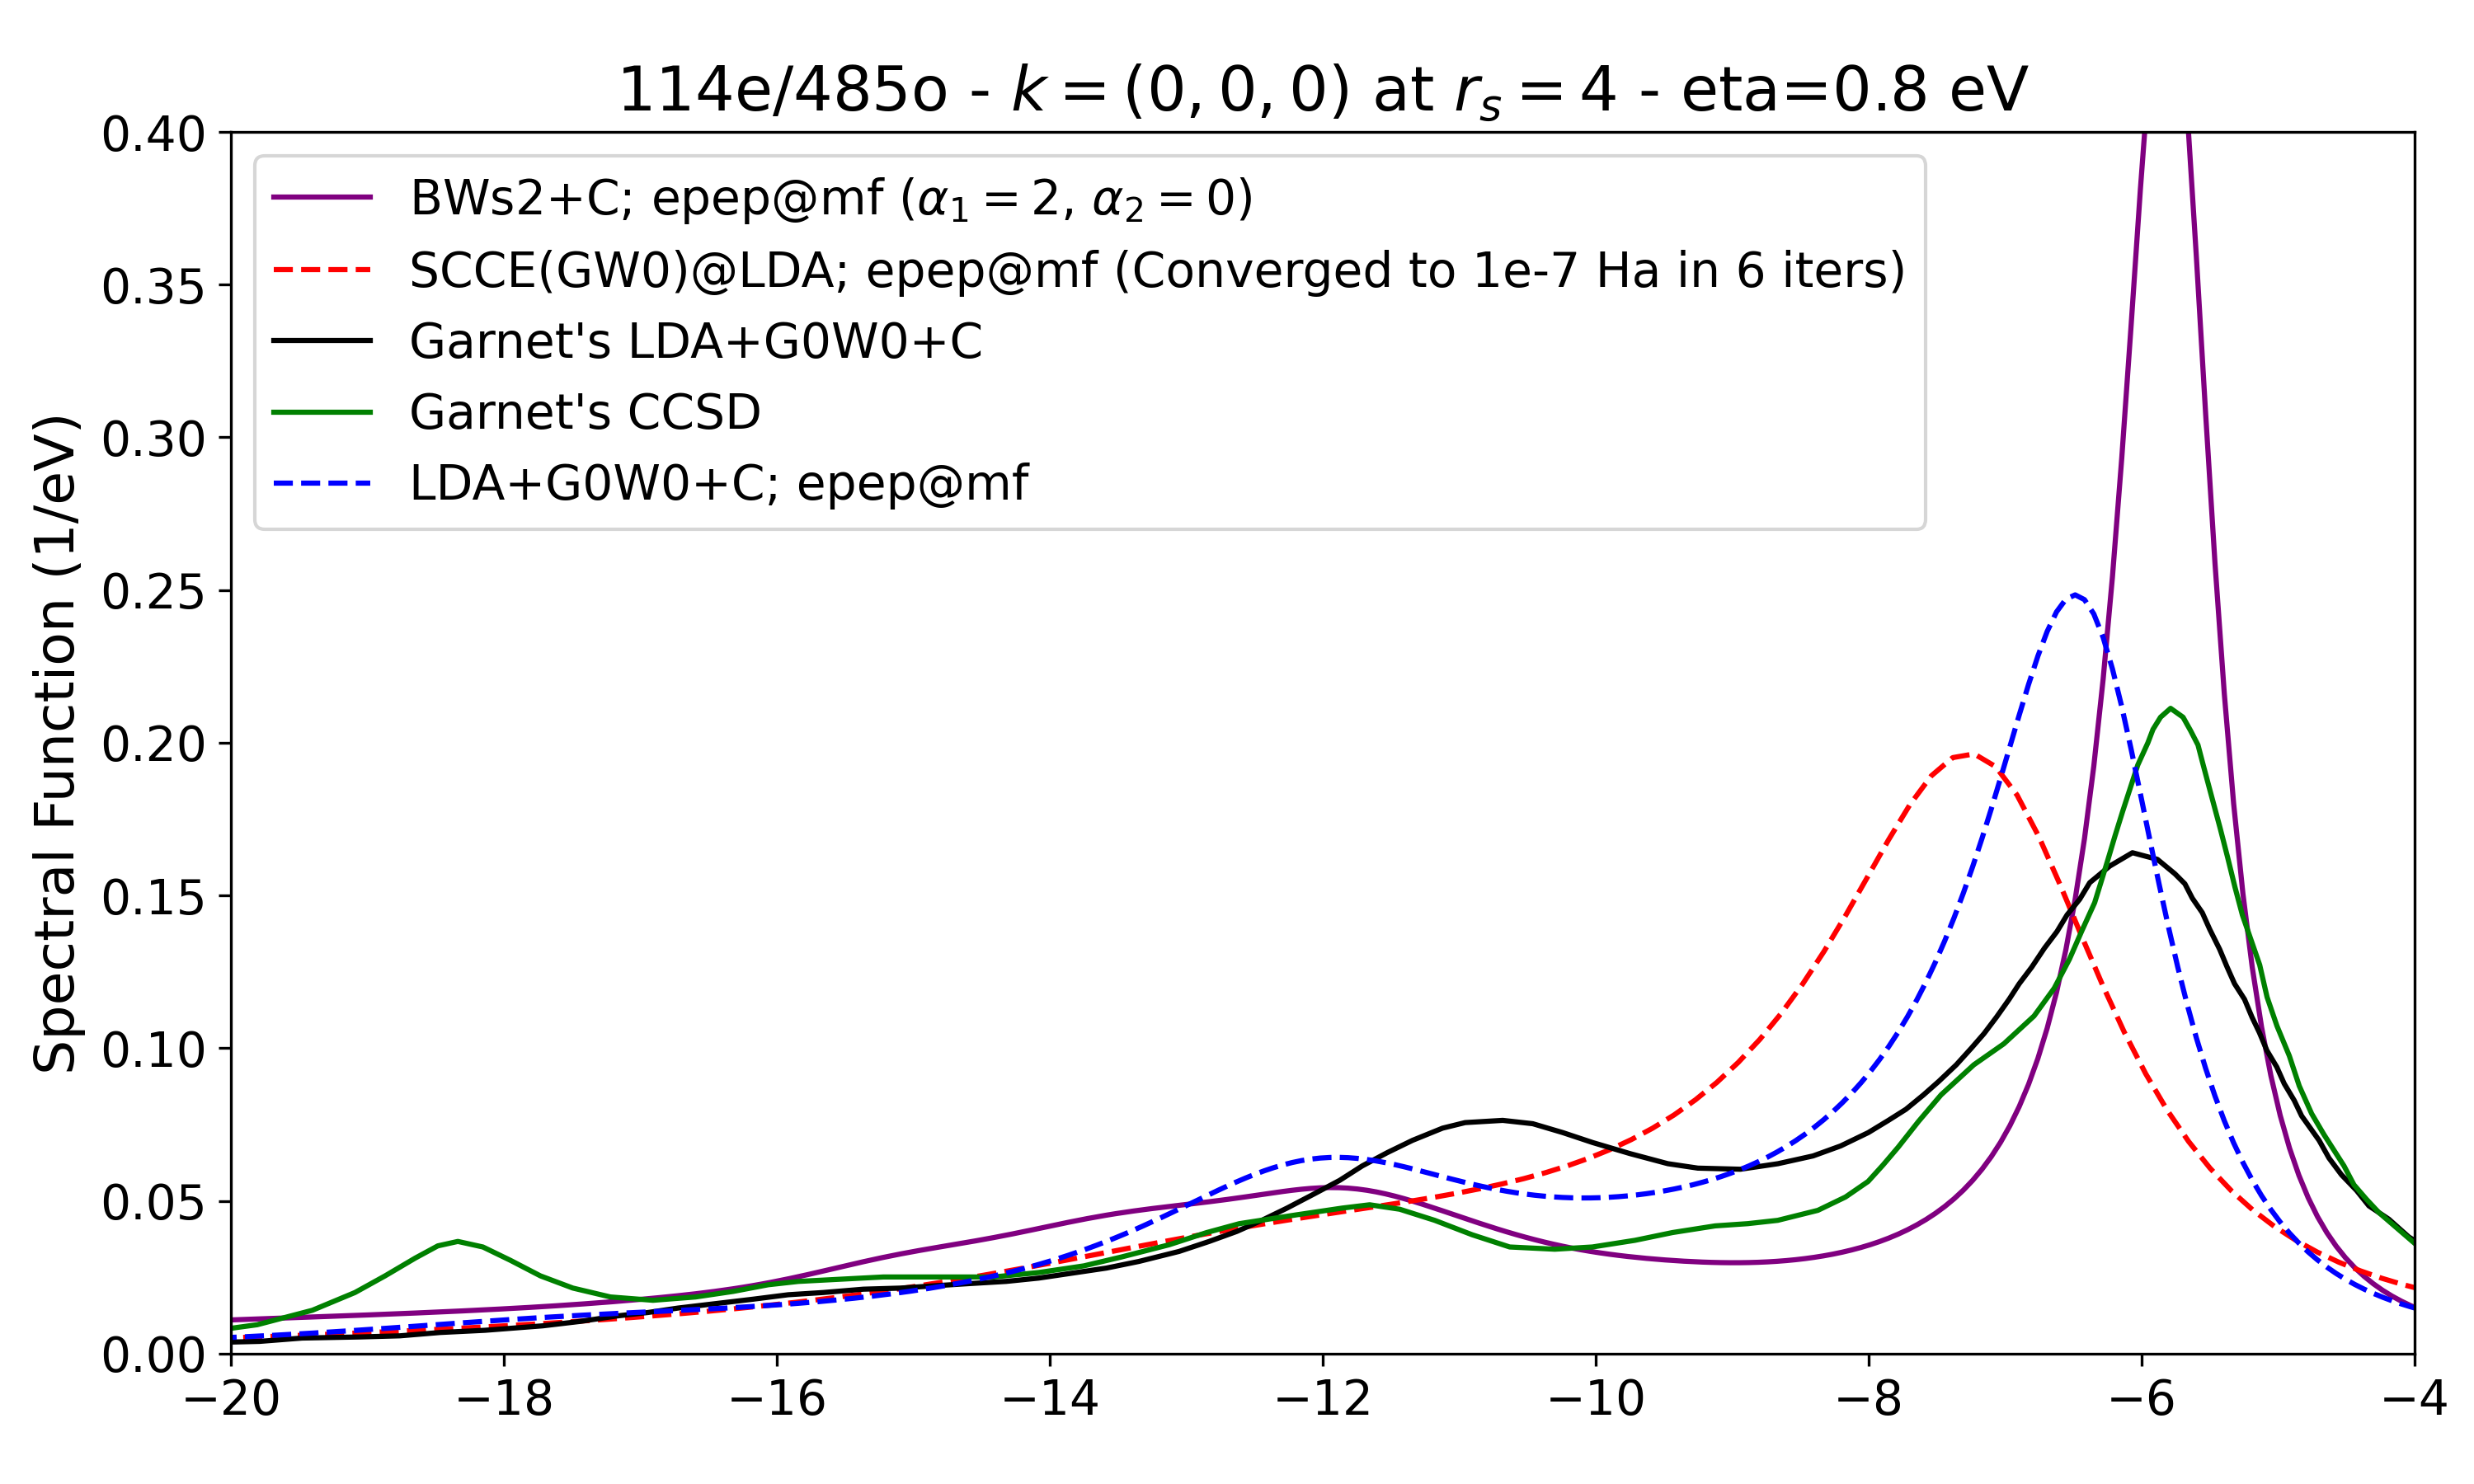
\includegraphics[width=\textwidth]{26/7/7-23/refpgw.png}
        % \caption{LDA+GW}
    \end{figure}
\end{frame}
\begin{frame}
    \frametitle{Notes on SCCE(GW0)}
Holm updates the self energy as:
\begin{equation}
\Sigma^{c}(\mathbf{k}, \omega)=\int_C \frac{\Gamma\left(\mathbf{k}, \omega^{\prime}\right)}{\omega-\omega^{\prime}} d \omega^{\prime}
\end{equation}
where
\begin{align}
\Gamma(\mathbf{k}, \omega)&=\sum_{\mathbf{q}} \int_0^\omega d \omega^{\prime} A\left(\mathbf{k}+\mathbf{q}, \omega-\omega^{\prime}\right) B_0\left(\mathbf{q}, \omega^{\prime}\right) \\
    A(k, \omega)&=\sum_\nu \frac{W_\nu(k)}{\sqrt{2 \pi \Gamma_\nu(k)}} \exp \left[-\frac{\left[\omega-E_\nu(k)\right]^2}{2 \Gamma_\nu^2(k)}\right].
\end{align}
\pause 
I do
\begin{equation}
    \Sigma_{m}^{c,R}(t)=\theta(t) \sum_{n I}\left|M_{ m,n}^I\right|^2\left[G_{n,CE}^{>}(t) e^{-i \Omega_I t}-G_{n,CE}^{<}(t) e^{+i \Omega_I t}\right].
\label{eq:scce_gw0}
\end{equation}
\end{frame}
% \begin{frame}
%     \frametitle{Implementation details}

%     \begin{itemize}
%         \item Casida diagonalization is preferred for G0W0+C
%         \pause
%         \item 2007o is pushing towards the limit of feasible basis size
%         \pause 
%         \end{itemize}
% \end{frame}
\section{Connection to CCGF}
\begin{frame}
    \frametitle{Ground State of the Electronic Polaron in the IBM}
Hamiltonian is 
\begin{equation}
H_{\rm ch}
=
E_{\rm ch}
+
\sum_\nu
\Omega_\nu Q_\nu^\dagger Q_\nu
+
\sum_\nu
\left(
M_\nu Q_\nu^\dagger
+
M_\nu^* Q_\nu
\right).
\end{equation}
\pause
The RPA ground state is a coherent state of QB operators $Q_\nu$ as
\begin{equation}
    |\Theta_{ch}\rangle = D(\beta)\left|0_{\mathrm{RPA}}\right\rangle.
\end{equation} 
\pause
The displacement operator is defined as
\begin{equation}
    D(\beta)=\exp \left[\sum_\mu\left(\beta_\mu Q_\mu^{\dagger}-\beta_\mu^* Q_\mu\right)\right] .
\end{equation}
where $\beta_\mu = -M_\mu / \Omega_\mu$.
\end{frame}
\begin{frame}
    \frametitle{Green's function of the electronic polaron}
Using the shifted QB operators
\begin{equation}
\widetilde Q_\nu
=
Q_\nu
- \beta_\nu
\qquad
\widetilde Q_\nu^\dagger
=
Q_\nu^\dagger
+
\beta_\nu^*,
\end{equation}
of which $\left|0_{\mathrm{RPA}}\right\rangle$ is a coherent state,
\pause we can rewrite the Hamiltonian as
\begin{equation}
H_{\rm ch}
=
E_{\rm pol}
+
\sum_\nu
\Omega_\nu
\widetilde Q_\nu^\dagger \widetilde Q_\nu ,
\end{equation}
where $E_{\rm pol}=E_{\rm ch}-\sum_\nu \Omega_\nu |\beta_\nu|^2$. \pause Then
\begin{align}
G^{QB,R}_{\rm ch}(t)
&=
-i \theta(t)
\left\langle 0_{\rm RPA} \right|
e^{-i H_{\rm ch} t}
\left|0_{\rm RPA}\right\rangle
\\
% &=-i \theta(t) e^{-i E_{\mathrm{pol}} t}\left\langle 0_{\mathrm{RPA}}\right| e^{-i \sum_\nu \Omega_\nu \tilde{Q}_\nu \tilde{Q}_\nu t}\left|0_{\mathrm{RPA}}\right\rangle \label{eq:G_ch_t} \\
% &=
% -i \theta(t)
% e^{-i E_{\rm pol} t}
% \exp
% \left[
% \sum_{\nu}
% |\beta_{\nu}|^2
% \left(
% e^{-i \Omega_{\nu} t}
% -
% 1
% \right)
% \right]
% \\
&=
-i \theta(t)
e^{-i E_{\rm pol} t}
\underbrace{
\exp
\left[
-\sum_{\nu} |\beta_{\nu}|^2
\right]
}_{Z_{\rm pol}}
\prod_{\nu}
\exp
\left[
|\beta_{\nu}|^2 e^{-i\Omega_{\nu} t}
\right]
\\
% &=
% -i \theta(t)
% Z_{\rm pol}
% e^{-i E_{\rm pol} t}
% \prod_{\nu}
% \sum_{n_{\nu}=0}^{\infty}
% \frac{
% |\beta_{\nu}|^{2n_{\nu}}
% }{
% n_{\nu}!
% }
% e^{-i n_{\nu} \Omega_{\nu} t}
% \\
&=
-i \theta(t)
Z_{\rm pol}
\sum_{\mathbf n}
\left[
\prod_{\nu}
\frac{
|\beta_{\nu}|^{2n_{\nu}}
}{
n_{\nu}!
}
\right]
\exp
\left[
-i
\left(
E_{\rm pol}
+
\sum_{\nu} n_{\nu}\Omega_{\nu}
\right)t
\right].
\end{align}
\end{frame}
\begin{frame}
    \frametitle{Connection between the cumulant and the CCGF in this formalism}
If instead of the IBM, we consider
\begin{equation}
H_p^{\rm eff}
=
\epsilon_p^{\rm HF}
+
\sum_{m\nu}
\Delta_{pm\nu}
B_{pm\nu}^{\dagger}
B_{pm\nu}
+
\sum_{m\nu}
\left(
\mathcal{M}_{pm\nu}
B_{pm\nu}^{\dagger}
+
\mathcal{M}_{pm\nu}^{*}
B_{pm\nu}
\right),
\end{equation}

then we recover the G0W0+C Green's function. \pause We can make contact with the CCGF, by instead considering the Hamiltonian
\begin{equation}
H_{\mathrm{ch}}=E_{\mathrm{ref}}^{\mathrm{ch}}+\sum_{p q} f_{p q}^{\mathrm{ch}}\left\{a_p^{\dagger} a_q\right\}+\frac{1}{4} \sum_{p q r s} v_{p q r s}^{\mathrm{ch}}\left\{a_p^{\dagger} a_q^{\dagger} a_s a_r\right\},
\end{equation}
which leads to the CCGF.
\end{frame}
